
\documentclass{standalone}
\usepackage{tikz}
\usepackage{fp}
\begin{document}
    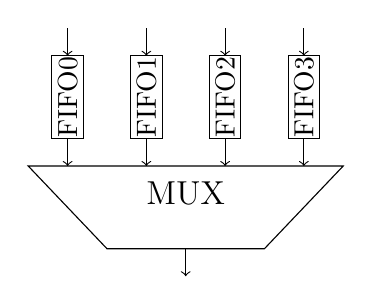
\begin{tikzpicture}[yscale=.7]
        \draw (-2,1) -- (2,1) -- (1,-.5) -- (-1,-.5) -- cycle;
        \node at (0,.5){\large MUX};
        \draw [->](0,-.5) -- (0,-1);
        \foreach [count=\c] \i in {-1.5, -.5, ..., 1.5}{
            \FPeval{\cm}{round(\c-1:0)};
            \draw (\i-.2,1.5) rectangle (\i+.2,3);
            \node at (\i,2.25)[rotate=90]{FIFO\cm};
            \draw [->](\i,1.5) -- (\i,1);
            \draw [->](\i,3.5) -- (\i,3);
        }
    \end{tikzpicture}
    \end{document}
